


% Default to the notebook output style


% Inherit from the specified cell style.




    
\documentclass{report}

    
    

    \usepackage{graphicx} % Used to insert images
    \usepackage{adjustbox} % Used to constrain images to a maximum size 
    \usepackage{color} % Allow colors to be defined
    \usepackage{enumerate} % Needed for markdown enumerations to work
    \usepackage{geometry} % Used to adjust the document margins
    \usepackage{amsmath} % Equations
    \usepackage{amssymb} % Equations
    \usepackage[mathletters]{ucs} % Extended unicode (utf-8) support
    \usepackage[utf8x]{inputenc} % Allow utf-8 characters in the tex document
    \usepackage{fancyvrb} % verbatim replacement that allows latex
    \usepackage{grffile} % extends the file name processing of package graphics 
                         % to support a larger range 
    % The hyperref package gives us a pdf with properly built
    % internal navigation ('pdf bookmarks' for the table of contents,
    % internal cross-reference links, web links for URLs, etc.)
    \usepackage{hyperref}
    \usepackage{longtable} % longtable support required by pandoc >1.10
    
\usepackage[round]{natbib}
\usepackage[doublespacing]{setspace}
\usepackage{parskip}


    
    \definecolor{orange}{cmyk}{0,0.4,0.8,0.2}
    \definecolor{darkorange}{rgb}{.71,0.21,0.01}
    \definecolor{darkgreen}{rgb}{.12,.54,.11}
    \definecolor{myteal}{rgb}{.26, .44, .56}
    \definecolor{gray}{gray}{0.45}
    \definecolor{lightgray}{gray}{.95}
    \definecolor{mediumgray}{gray}{.8}
    \definecolor{inputbackground}{rgb}{.95, .95, .85}
    \definecolor{outputbackground}{rgb}{.95, .95, .95}
    \definecolor{traceback}{rgb}{1, .95, .95}
    % ansi colors
    \definecolor{red}{rgb}{.6,0,0}
    \definecolor{green}{rgb}{0,.65,0}
    \definecolor{brown}{rgb}{0.6,0.6,0}
    \definecolor{blue}{rgb}{0,.145,.698}
    \definecolor{purple}{rgb}{.698,.145,.698}
    \definecolor{cyan}{rgb}{0,.698,.698}
    \definecolor{lightgray}{gray}{0.5}
    
    % bright ansi colors
    \definecolor{darkgray}{gray}{0.25}
    \definecolor{lightred}{rgb}{1.0,0.39,0.28}
    \definecolor{lightgreen}{rgb}{0.48,0.99,0.0}
    \definecolor{lightblue}{rgb}{0.53,0.81,0.92}
    \definecolor{lightpurple}{rgb}{0.87,0.63,0.87}
    \definecolor{lightcyan}{rgb}{0.5,1.0,0.83}
    
    % commands and environments needed by pandoc snippets
    % extracted from the output of `pandoc -s`
    
    \DefineShortVerb[commandchars=\\\{\}]{\|}
    \DefineVerbatimEnvironment{Highlighting}{Verbatim}{commandchars=\\\{\}}
    % Add ',fontsize=\small' for more characters per line
    \newenvironment{Shaded}{}{}
    \newcommand{\KeywordTok}[1]{\textcolor[rgb]{0.00,0.44,0.13}{\textbf{{#1}}}}
    \newcommand{\DataTypeTok}[1]{\textcolor[rgb]{0.56,0.13,0.00}{{#1}}}
    \newcommand{\DecValTok}[1]{\textcolor[rgb]{0.25,0.63,0.44}{{#1}}}
    \newcommand{\BaseNTok}[1]{\textcolor[rgb]{0.25,0.63,0.44}{{#1}}}
    \newcommand{\FloatTok}[1]{\textcolor[rgb]{0.25,0.63,0.44}{{#1}}}
    \newcommand{\CharTok}[1]{\textcolor[rgb]{0.25,0.44,0.63}{{#1}}}
    \newcommand{\StringTok}[1]{\textcolor[rgb]{0.25,0.44,0.63}{{#1}}}
    \newcommand{\CommentTok}[1]{\textcolor[rgb]{0.38,0.63,0.69}{\textit{{#1}}}}
    \newcommand{\OtherTok}[1]{\textcolor[rgb]{0.00,0.44,0.13}{{#1}}}
    \newcommand{\AlertTok}[1]{\textcolor[rgb]{1.00,0.00,0.00}{\textbf{{#1}}}}
    \newcommand{\FunctionTok}[1]{\textcolor[rgb]{0.02,0.16,0.49}{{#1}}}
    \newcommand{\RegionMarkerTok}[1]{{#1}}
    \newcommand{\ErrorTok}[1]{\textcolor[rgb]{1.00,0.00,0.00}{\textbf{{#1}}}}
    \newcommand{\NormalTok}[1]{{#1}}
    
    % Define a nice break command that doesn't care if a line doesn't already
    % exist.
    \def\br{\hspace*{\fill} \\* }
    % Math Jax compatability definitions
    \def\gt{>}
    \def\lt{<}
    % Document parameters
    
\title{The white matter disonnection syndrome in neurocognitive ageing}

    
\date{\today}

    
\author{John David Griffiths}

    

    
    % Prevent overflowing lines due to hard-to-break entities
    \sloppy
    % Setup hyperref package
    \hypersetup{
      breaklinks=true, % so long urls are correctly broken across lines
      hidelinks
      }
    % Slightly bigger margins than the latex defaults
    \geometry{verbose,tmargin=1in,bmargin=1in,lmargin=1in,rmargin=1in}
    
    %\parskip=2\baselineskip \advance\parskip by 0pt plus 20pt
    \setlength{\parskip}{0pt} % 1ex plus 0.5ex minus 0.2ex}
    \setlength{\parindent}{0pt}



    \begin{document}
    
    
    
    \maketitle
    
    
    \tableofcontents


    

    {Mock Chapter 1}



    \chapter{An enchanting mock chapter 1 title goes here}


    \textbf{\emph{Abstract}}

    Important note about section headings:

In order to get both markdown (notebook) and latex playing ball, I: -
Use heading one in the notebook for Chapter number - Use heading two in
notebook for chapter title - Set chapter heading one block in nbconvert
template file to blank - \ldots{}result = heading ones are ommitted in
latex docs. Latex adds its own titles anyway (this is why I wanted to
sort this).

    Now: the question is - will things be excluded because they are in
markdown cells, of because of the nbconvert template.

Test:

\begin{itemize}
\item
  chapter sub title is current not in html tags and not blocked
\item
  \ldots{}but chapter number is in markdown
\item
  \ldots{}so: should be excluded in markdown
\end{itemize}

1: chapter 1 title and subtitle in heading 1, but chapter 1 number in
html 2 - chapter 1 in title and chapter 2 in subtitute - switch on
suppresion of chapter in nbconvert

    Lorem ipsum blah blah


    \section{Background}


    blah blah blah


    \section{Methods}


    blah blah blah

    \begin{figure}[htbp]
\centering
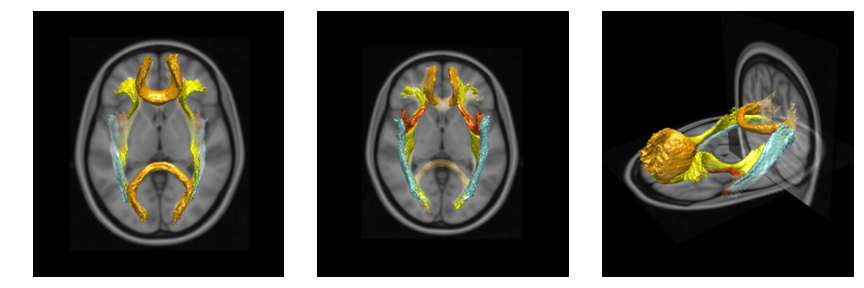
\includegraphics{figures/Ch2_JHU_tracts.png}
\caption{JHU tracts \{Adding a fuller caption which is what I woudl like
to say about the JHU tracts. Hopefuly this will not appear in the list
of figures. If the label tag does its job, I think that's what should
happen. But there's also this issue about closing the square
bracket\ldots{} \label{fig:JHU tracts}}
\end{figure}

HTML caption here - JHU tracts Adding a fuller caption which is what I
woudl like to say about the JHU tracts. Hopefuly this will not appear in
the list of figures. If the label tag does its job, I think that's what
should happen. But there's also this issue about closing the square
bracket\ldots{}

    blah blah blah


    \section{Results}


    blah blah blah

    \begin{figure}[htbp]
\centering
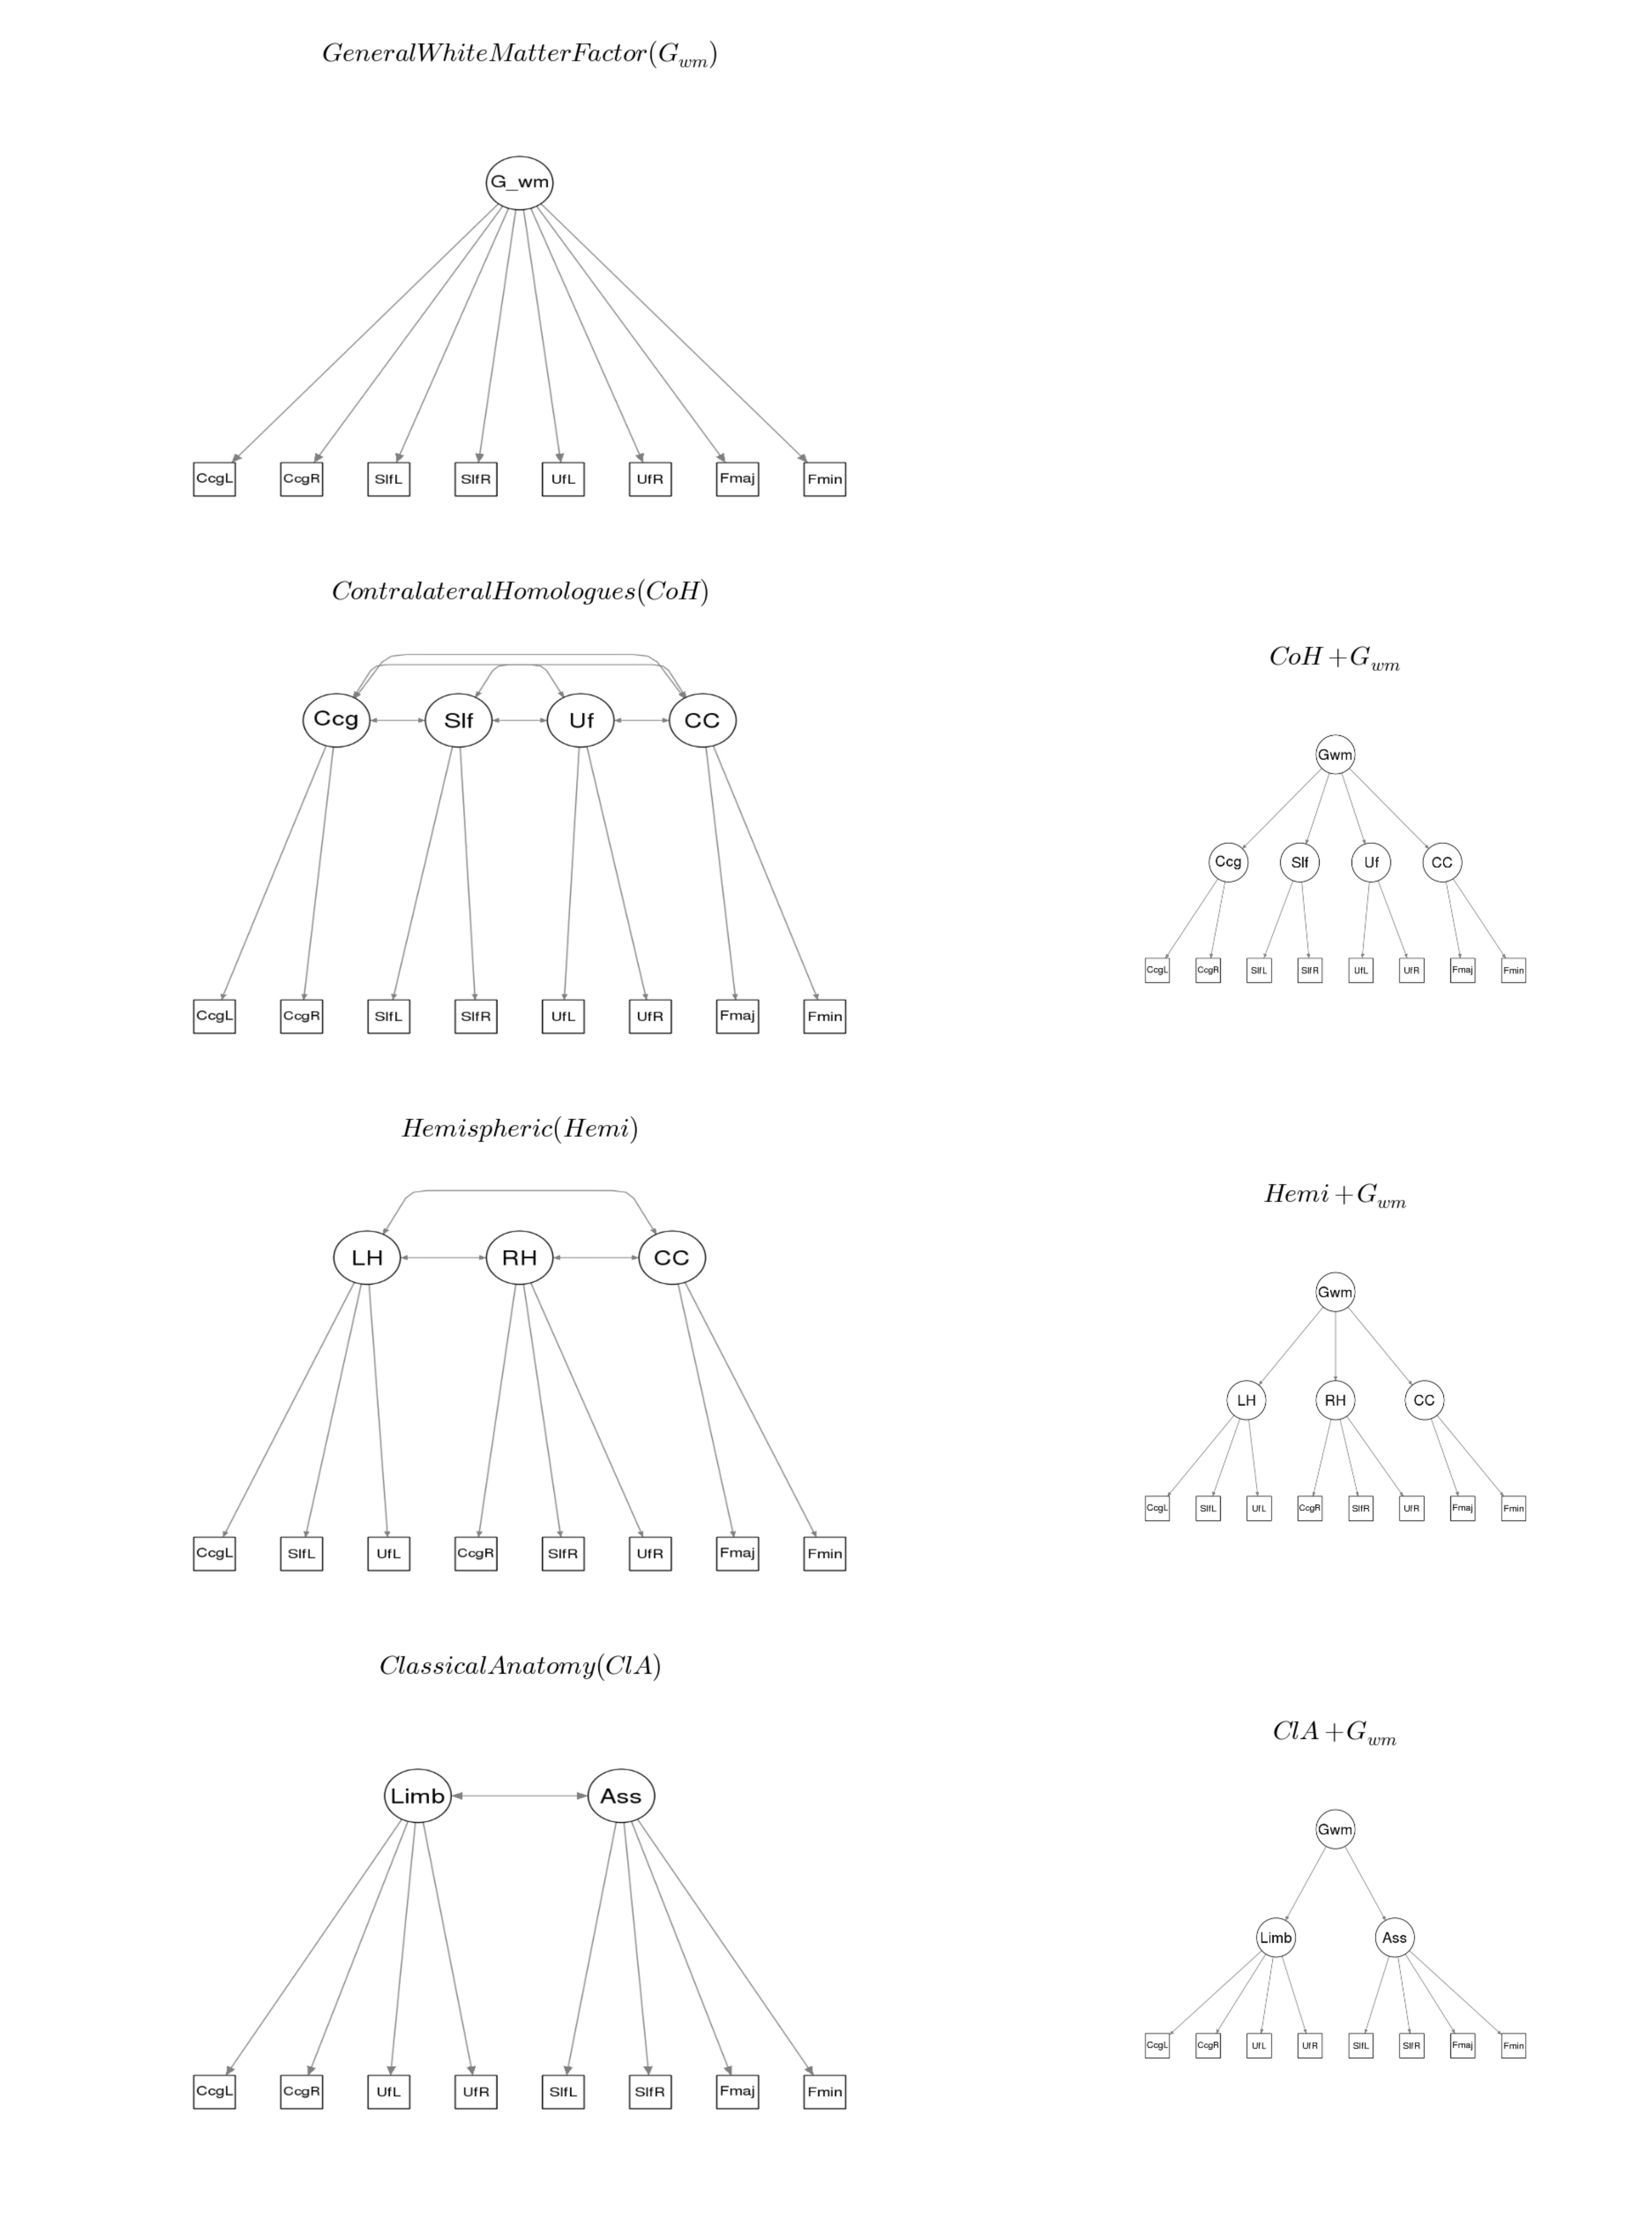
\includegraphics{figures/SEM_models.png}
\caption{SEM models \label{fig:SEM models}}
\end{figure}

HTML caption here - SEM models


    \section{Discussion}


    Minion hyperlink test

(see here
https://groups.google.com/forum/\#!msg/pandoc-discuss/MxGKvnNI08c/M6398LGWvqIJ)

    
\includegraphics{figures/minion.png}\{\#minion\}

HTML caption - minion (original pandoc hyperlink test)

    blah blah blah

    Alternative hyperlink test - see here:

\begin{verbatim}
http://stackoverflow.com/questions/9434536/how-do-i-make-a-reference-to-a-figure-in-markdown-using-pandoc
\end{verbatim}

    \begin{figure}[htbp]
\centering
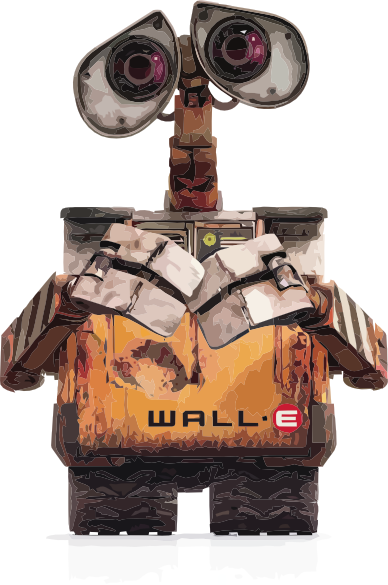
\includegraphics{figures/WallE.png}
\caption{WallE\label{fig:WallE}}
\end{figure}

Wall E HTML caption goes here; shouldn't be see by latex.

    blah blah blah

    \begin{figure}[htbp]
\centering

\includegraphics{figures/TomandJerry.png}
\caption{TomandJerry\label{fig:TomandJerry}}
\end{figure}

HTML caption here

    blah blah blah




    {Mock Chapter 2}



    \chapter{Add an exciting chapter 2 sub heading here\textgreater{}}


    \textbf{\emph{Abstract}}

    Important note about section headings:

In order to get both markdown (notebook) and latex playing ball, I: -
Use heading one in the notebook for Chapter number - Use heading two in
notebook for chapter title - Set chapter heading one block in nbconvert
template file to blank - \ldots{}result = heading ones are ommitted in
latex docs. Latex adds its own titles anyway (this is why I wanted to
sort this).

    Lorem ipsum blah blah


    \chapter{Background}


    blah blah blah


    \chapter{Methods}


    blah blah blah

    blah blah blah


    \chapter{Results}


    blah blah blah

    \begin{figure}[htbp]
\centering
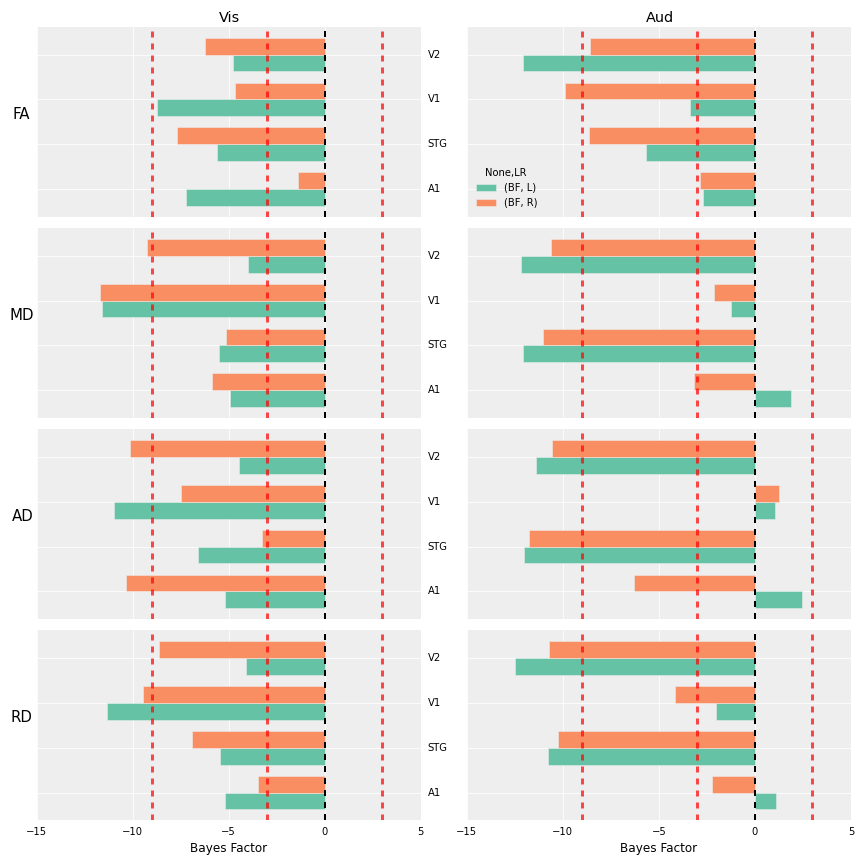
\includegraphics{figures/dwi_mediation_of_age_fx_on_onset_latency_bayesfactors.png}
\caption{Bayes Factors \label{fig:Bayes factors}}
\end{figure}

HTML caption here - Bayes factors


    \chapter{Discussion}


    blah blah blah


    {Mock Chapter 3}



    \chapter{The exciting sub heading chapter name of mock chapter 3}


    \textbf{\emph{Abstract}}

    blah blah blah\\blah blah blah\\blah blah blah\\blah blah blah\\blah
blah blah

    Lorem ipsum blah blah


    \chapter{Background}


    blah blah blah


    \chapter{Methods}


    blah blah blah

    \begin{figure}[htbp]
\centering
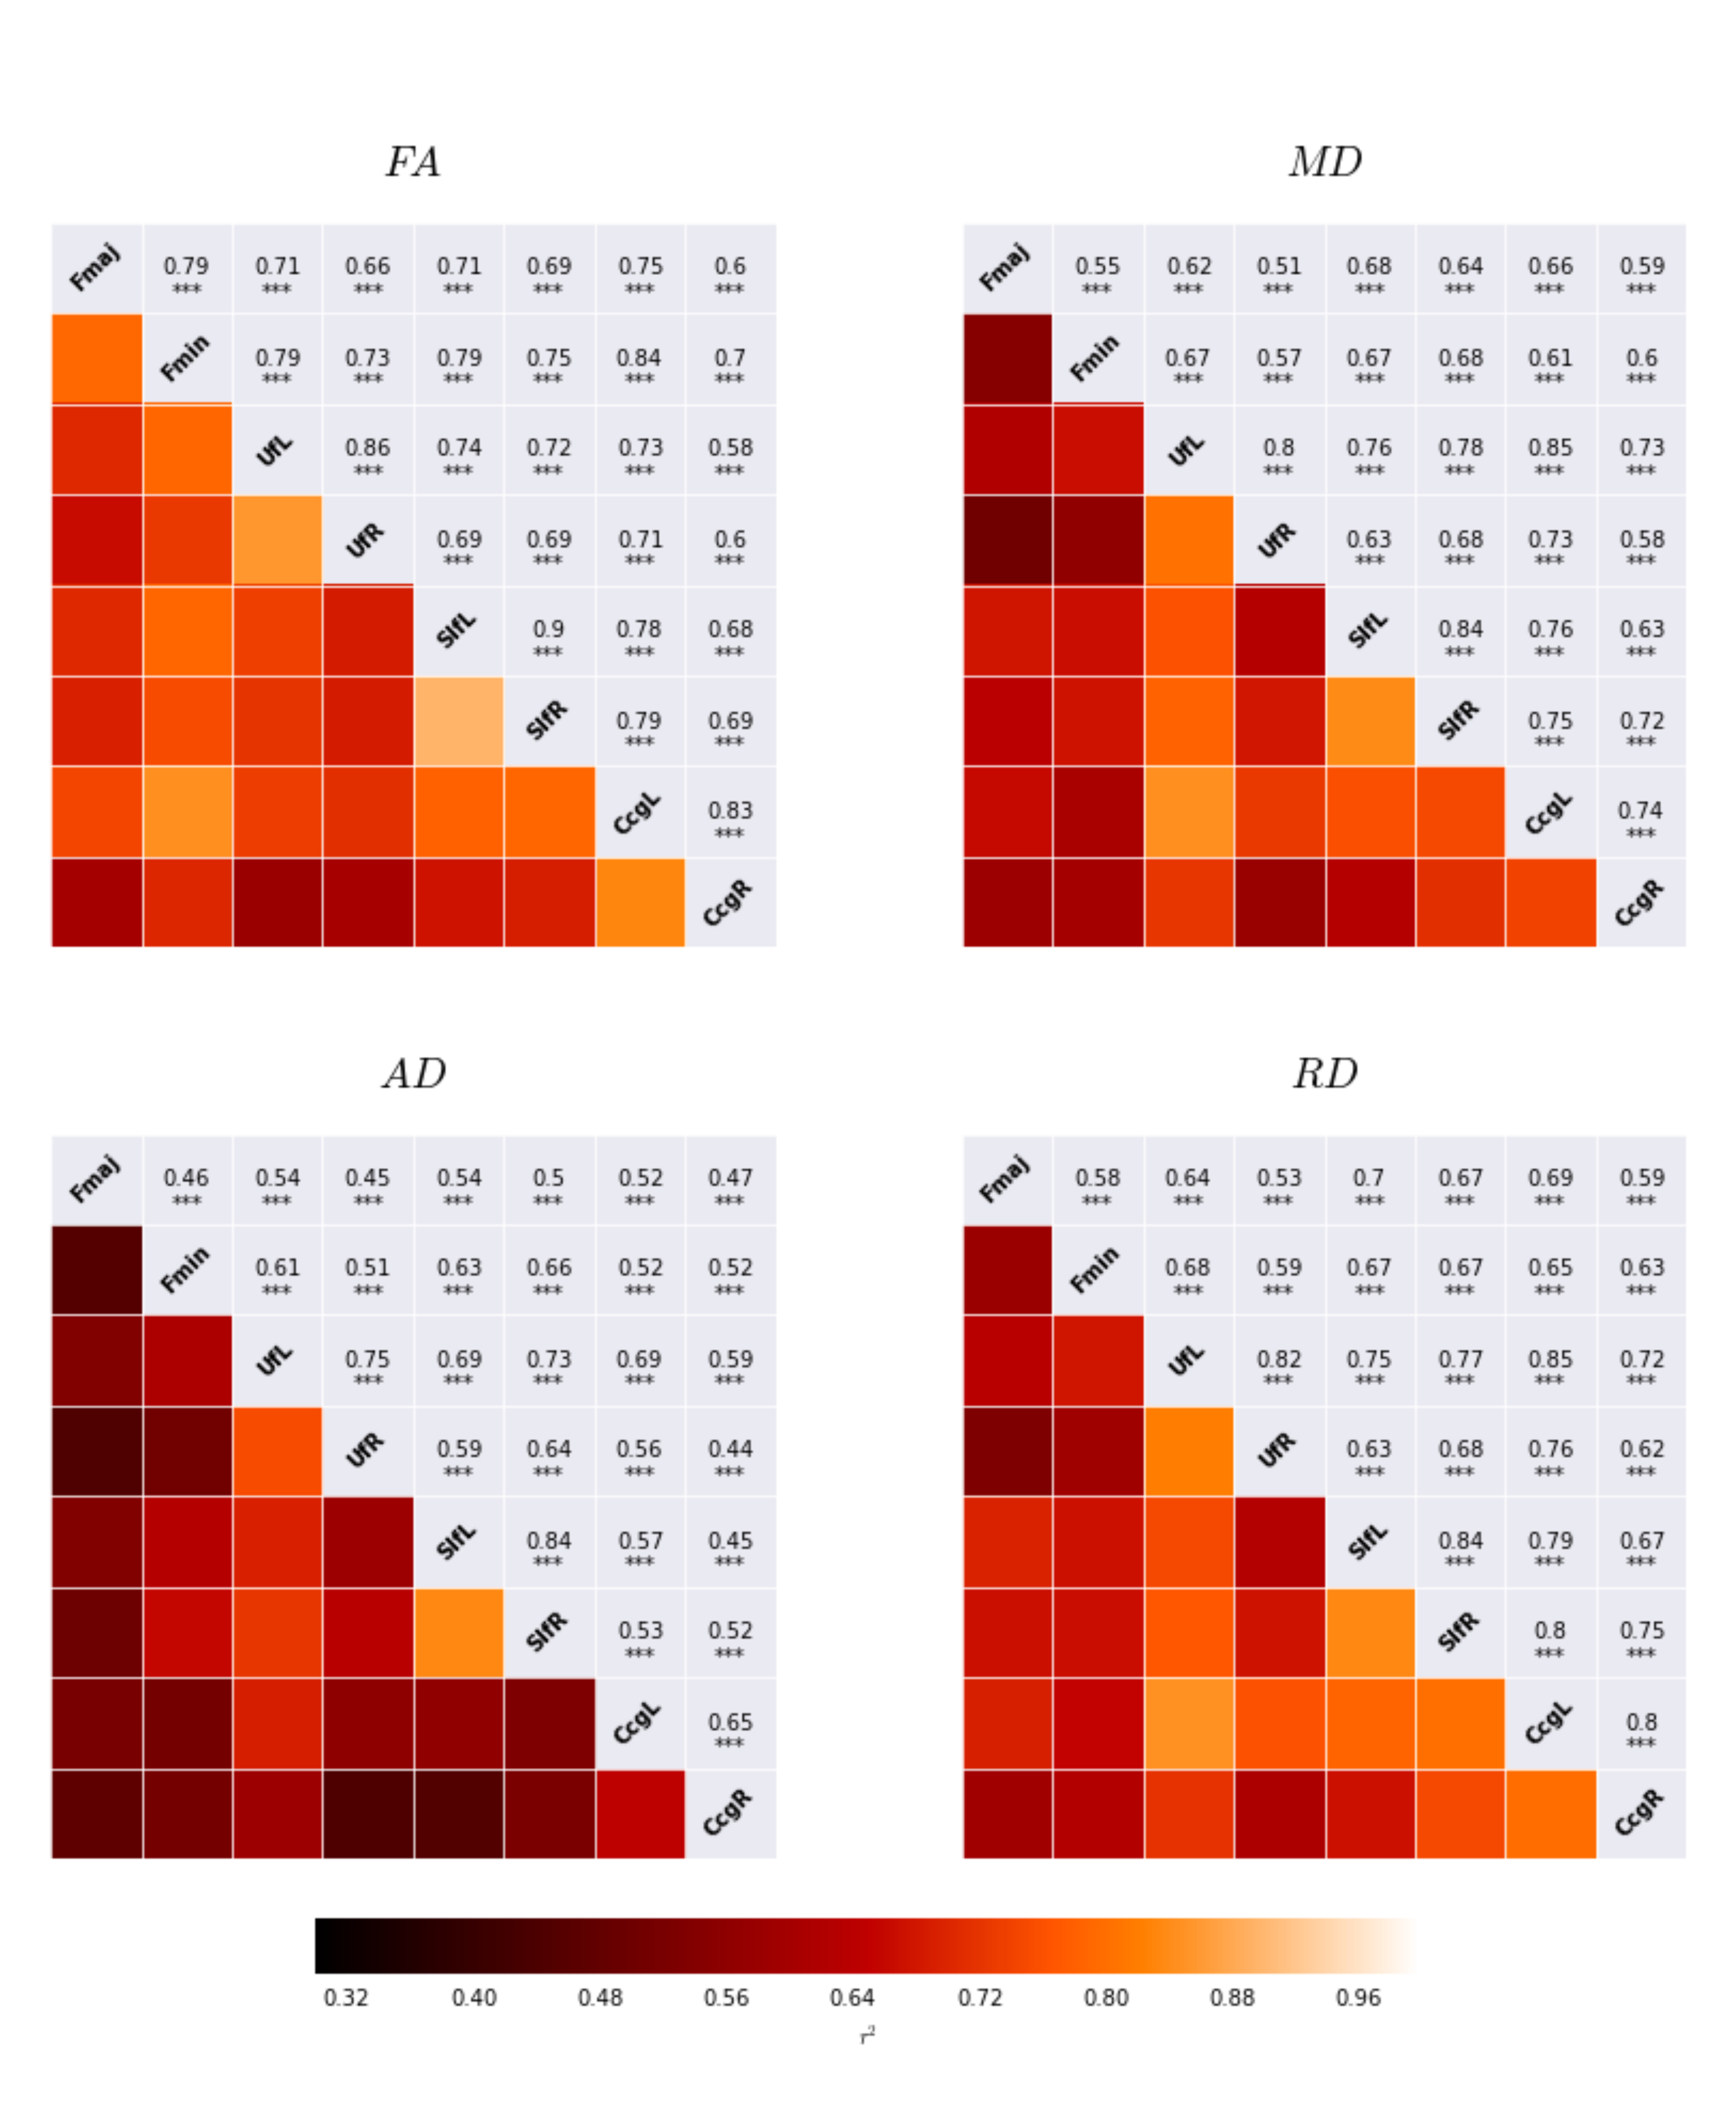
\includegraphics{figures/f2p5_correlations_table.png}
\caption{Correlations /label\{fig:correlations\}}
\end{figure}

HTML caption - correlations

    blah blah blah


    \chapter{Results}


    blah blah blah


    \chapter{Discussion}


    blah blah blah



    % Add a bibliography block to the postdoc
    
    
\bibliographystyle{apalike}
\bibliography{Thesis}

    
    \end{document}
